\section{Security and Privacy Analysis}
\label{sec:analysis}
%In this section, we analyze the security and privacy guarantees provided by \usso.
We define different adversarial scenarios against the security and privacy guarantees provided by UPPRESSO,
    develop a  Dolev-Yao style model to analyze the login flow,
    and formally prove each of these guarantees in respective scenarios based on the conditions confirmed in the model.

\subsection{Adversarial Scenarios}

Based on our design goals and the potential adversaries discussed in Section \ref{subsec:threatmodel},
we consider three adversarial scenarios as below,
    and then the security and privacy guarantees of UPPRESSO are proved in respective scenarios.

\noindent\textbf{Security.}
Malicious users could colludes with each other or with malicious RPs,
    attempting to impersonate an honest user to login to an honest RP or entice an honest user to login to an honest RP under another user's account.

\noindent\textbf{Privacy against the IdP.}
The honest-but-curious IdP tries to infer the identities of the RPs that a user requests to access.
   %     or link multiple login instances to any RP that initiated by a user.

\noindent\textbf{Privacy against RPs.}
Malicious RPs collude with each other or with malicious users,
 attempting to link login instances across these RPs that initiated by a user.


% \textcolor{blue}{Based on the threat model and assumptions proposed in Section \ref{sec:UPPRESSO},
%     different types of adversaries are considered in the analysis of security and privacy.
% First of all, in the proofs of security,
%     malicious RPs collude with malicious users,
%         attempting
%         to break any of the four security properties of SSO identity tokens for an honest user to visit an honest RP.
% Then, in the analysis of privacy against the IdP-based login tracing,
%    an honest-but-curious IdP is the only adversary.
% Finally,
%     in the privacy analysis against the RP-based identity linkage,
%     a number of malicious RPs collude, attempting to link an honest user's accounts across these RPs.}

% We first analyzed UPPRESSO %especially confidentiality and integrity,
%      based on a Dolev-Yao-style model \cite{SPRESSO}.
% % which has been used in the formal analysis of SSO protocols such as OAuth 2.0 \cite{FettKS16} and OIDC \cite{FettKS17}.
% The model abstracts the entities in a web system,
%     such as web servers and browsers,
%     as \emph{atomic processes}. %which communicate with each other through events. % such as HTTPS request and response.
% It defines \emph{script processes} to formulate client-side scripts.
% %The script is dependently invoked by the browser to process the server-defined logic.
%   %such as verifying $Certificate_{RP}$.
% %
% %postmessage events;
% %
% %atomic process <-> script process, communication.
% %
% %Other events change self-trigger.
% %
% UPPRESSO contains atomic processes including:
% an IdP process,
%     a finite set of web servers for honest RPs, a finite set of honest browsers, and a finite set of attacker processes.
% The processes communicate with each other through events such as HTTPS requests and responses.
% %We consider all RP and browser processes are honest,
% An RP or a browser controlled by adversaries is modeled as an attacker process.
% Within a browser,
%  an honest IdP script, an honest RP script, and also attacker scripts which are downloaded from attacker processes,
%   are invoked.
% %Although the scripts coexist in the same browser, they are strictly separated.
% Script processes communicate with each other through \verb+postMessage+,
%     modelled as transmitted-to-itself events of a browser process.
% %To clearly indicate the action of postMessage communication, we define it as the transmitting-to-itself event of the browser (which is not defined in SPRESSO).


% \textcolor{blue}{After formulating the system by this model,
%     we analyze the following data for the proofs in Sections \ref{analysis-security} and \ref{sec-:analysis},
%      when there are corresponding adversaries.
% We (\emph{a}) trace the lifecycle of an identity token for an honest user to visit an honest RP,
%         starting when it is generated and ending when accepted by the RP,
%     to ensure it is not leaked to adversaries,
% (\emph{b})
%     locate all places
%         where $PID_U$, $PID_{RP}$ and other parameters enclosed in the token are processed,
%      to ensure no adversary able to manipulate them,
% and (\emph{c})
%     locate the places where $PK$ is transmitted and used in the IdP script,
%         to ensure no adversary tampering with it.
% These conclusions are used to prove security of the UPPRESSO protocols.}
% %
% % to ensure it is not leaked to attackers or tampered with by any adversary without checking.
% \textcolor{blue}{In the meantime,
%         this model ensures that (\emph{a}) $t$ is unaccessible to the honest-but-curious IdP,
%  which is necessary to prevent the IdP-based login tracing,
%  and (\emph{b}) $u$ and $r$ are not leaked to RPs in the protocols,
%     necessary to prevent the RP-based identity linkage.}


%Next, we prove that \usso~is secure in the first adversarial scenario in Section~\ref{analysis-security} and it can prevent privacy threats in the other two adversarial scenarios in Section~\ref{sec-:analysis}.

%======move to security analysis
%The RP cannot derive $ID_U$ from either $PID_U$ or $Acct$ due to the elliptic curve discrete logarithm problem (ECDLP). Since $t$ is random in $\mathbb{Z}_n$ and unknown to the IdP, from the IdP's view, $PID_{RP}$ is indistinguishable from a random variable on $\mathbb{E}$. So, the IdP cannot learn anything about $ID_{RP}$ from $PID_{RP}$.
%Section \ref{sec:analysis} presents more detailed analyses.

\subsection{The Dolev-Yao-Style Model for UPPRESSO}
\label{dy-model}
We develop a Dolev-Yao-style model \cite{SPRESSO},
    referred to as the \emph{DYU model},
to formalize the login flow of UPPRESSO. % which has been used in the formal analysis of SSO protocols such as OAuth 2.0 \cite{FettKS16} and OIDC \cite{FettKS17}.
It abstracts the entities in a web system, such as web servers and browsers, as \emph{atomic processes} %which communicate with each other through events. % such as HTTPS request and response.
and defines \emph{script processes} to formulate client-side scripts.
%The script is dependently invoked by the browser to process the server-defined logic.%such as verifying $Certificate_{RP}$. %postmessage events; %atomic process <-> script process, communication. %Other events change self-trigger.
Thus, the atomic processes of \usso~include an {\em IdP process}, a finite set of {\em web servers} for honest RPs, a finite set of honest {\em browsers}, and a finite set of {\em attacker processes} that model malicious RPs and malicious users. The processes communicate with each other through events such as HTTPS requests and responses.
A browser may invoke an honest IdP script and multiple RP scripts that could be honest or malicious.
%Although the scripts coexist in the same browser, they are strictly separated.
The script processes communicate with each other through \verb+postMessage+, which are modeled as transmitted-to-itself events of a browser process.
%To clearly indicate the action of postMessage communication, we define it as the transmitting-to-itself event of the browser (which is not defined in SPRESSO).

\newc
With the DYU model, we (\emph{a}) trace the lifecycle of an identity token from its generation at the IdP to its acceptance at an RP, to prove that it cannot be leaked to adversaries;
(\emph{b}) locate the places where $PID_U$, $PID_{RP}$, and other elements in the identity token are processed,
 to prove that they cannot be manipulated by any adversary; and (\emph{c}) locate the places
  where $PK$ is transmitted and used in the IdP script,
to prove that it cannot be replaced by any adversary.
Meanwhile, we confirm that the IdP cannot learn anything about $t$ shared only between the user and the RP,
 while the RPs learn nothing about $u$ shared between the user and the IdP.
It is trivial to prove the confidentiality of $r$, as it never leaves the IdP.

\subsection{Security}
\label{analysis-security}

%A secure SSO system allows a \emph{legitimate} user to login to an \emph{honest} RP with her account at this RP,
% by presenting \emph{identity tokens} issued by a \emph{trusted} IdP.

We prove four properties of an identity token in UPPRESSO,
namely, RP designation, user identification, confidentiality and integrity,
and then prove that UPPRESSO is a secure SSO system based on these properties.

Let us consider an identity token $TK$ binding $PID_{RP}$ and $PID_U$, which is generated by the IdP upon a request from the authenticated user with $ID_U$.

%These conclusions are used to prove the security of the UPPRESSO protocols.
%We consider an arbitrary login instance in which an arbitrary RP with $ID_{RP}$ receives an integer $t$ and an identity token $TK$ issued by the IdP, binding a $PID_U$ and a $PID_{RP}$, from the RP script in a user browser. $TK$ is considered a valid identity token if the RP could verify its signature using the IdP's public key $PK$.

\vspace{1mm}
\noindent\textsc{Theorem 1. (RP Designation)} {\em $PID_{RP}$ in $TK$ uniquely designates an RP with $ID_{RP} = [r]G$,
 where $r$ is a random number known only to the IdP and $G$ is a generator on $\mathbb{E}$ of order $n$.}
%{\em Provided that $r$ is known only to the IdP, $PID_{RP}$ in the identity token uniquely designates the RP with $ID_{RP} = [r]G$.}}
%{\em If $TK$ is a valid identity token and $PID_{RP} = [t]ID_{RP}$ is satisfied, $PID_{RP}$ uniquely designates the RP that receives $TK$.}

\vspace{0.75mm}
\noindent\textsc{Proof.} We first prove that $PID_{RP}$ always specifies one RP in the system as below.
$PID_{RP}$ sent by the user in her identity-token request is calculated as $PID_{RP} = [t]ID_{RP}$,
 where $ID_{RP}$ is the target RP's identity and $t$ is a random number selected by the user and shared with this RP.
 Therefore, $PID_{RP}$ is associated with the target RP which receives $t$.

Next, according to Lemma 1, given $PID_{RP} = [t]ID_{RP}$, the probability of associating $PID_{RP}$ with another RP is negligible. This means that $PID_{RP}$ cannot be associated with any other RPs in the system. Therefore, $PID_{RP}$ designates only the target RP with $ID_{RP}$ in the system.  \hfill $\square$

\vspace{1mm}
\noindent\textsc{Lemma 1.} {\em  For any two RPs in a finite set of RPs, the probability of finding different numbers $t$ and $t'$ in $[1,n)$ that satisfy $[t]ID_{RP_j} = [t']ID_{RP_{j'}}$ is negligible, where $ID_{RP_j}=[r]G$, $ID_{RP_{j'}}=[r']G$, $r$ and $r'$ are different numbers unknown to the RPs, and $G$ is a generator on $\mathbb{E}$ of order $n$.}

%Based on the ECDLP we prove that, for adversaries, the probability of finding $t$ and $t'$ satisfying $[t]ID_{RP_j} = [t']ID_{RP_{j'}}$ is negligible, where $RP_j$ and $RP_{j'}$ are any two RPs in the finite set of RPs (i.e., $ID_{RP_j} = [r_j]G$ and $ID_{RP_{j'}} = [r_{j'}]G$, while $r_j$ and $r_{j'}$ are kept secret to the adversaries). This negligible probability means $PID_{RP_j} = [t]ID_{RP_j}$ designates \emph{only} the target RP with $ID_{RP_j}$.

\oldc
\vspace{0.75mm}
\noindent\textsc{Proof.}
Finding $t$ and $t'$ that satisfy $[t]ID_{RP_j} = [t']ID_{RP_{j'}}$, i.e., a $PID_{RP}$ collision,
    can be described as a game $\mathcal{G}_c$ between an adversary and a challenger: the adversary receives from the challenger a finite set of RP identities, i.e., $ID_{RP_1}$, ..., $ID_{RP_m}$, where $m$ is the number of RPs in the system, and outputs $(a, b, t, t')$ where $a \neq b$.
    If $[t]ID_{RP_a}=[t']ID_{RP_b}$, which occurs with a probability ${\rm Pr}_s$, the adversary succeeds in this game.
%The attack success probability is defined as ${\rm Pr}_s$.

Figure \ref{fig:ecdlp_algorithm} depicts a probabilistic polynomial time (PPT)  algorithm $\mathcal{D}^*_c$ based on $\mathcal{G}_c$,
    to solve the elliptic curve discrete logarithm problem (ECDLP):
find a number $x \in \mathbb{Z}_n$ satisfying $Q = [x]G$,
where $Q$ is a point on $\mathbb{E}$ and
    $G$ is a generator on $\mathbb{E}$ of order $n$.
The probability of solving this problem by any PPT algorithm $\mathcal{D}$ is defined as:
%For any PPT algorithm $\mathcal{D}$ is used to calculate $x$, we define the probability of finding $x$ as: %Therefore, the probability of finding $x$ using a probabilistic polynomial time (PPT) algorithm is negligible.
\begin{equation*}
{\rm Pr}\{\mathcal{D}(G, [x]G)=x\} = \epsilon_{c}(k)
\end{equation*}
%where ${\rm Pr}\{\}$ denotes the probability.
where $k$ denotes the security parameter. The probability, i.e. $\epsilon_{c}(k)$, becomes negligible when $k$ is sufficiently large.
%For any sufficiently large $k$, $m \ll 2^k$ since $m$ is a finite integer.


The input of $\mathcal{D}^*_c$ is in the form of ($G, Q$).
Upon receiving an input ($G$, $Q$), the challenger first randomly chooses $r_1, \cdots, r_m$ in $\mathbb{Z}_n$ to calculate $[r_1]G, \cdots, [r_m]G$, randomly replaces $[r_j]G$ with $Q$, and sends $m$ RP identities to the adversary, which then returns the result ($a$, $b$, $t$, $t'$).
Finally, the challenger calculates $s = t^{-1}t'r_b \bmod n$, and returns $s$ as the output of $\mathcal{D}^*_c$.

\begin{figure}[tb]
  \centering
  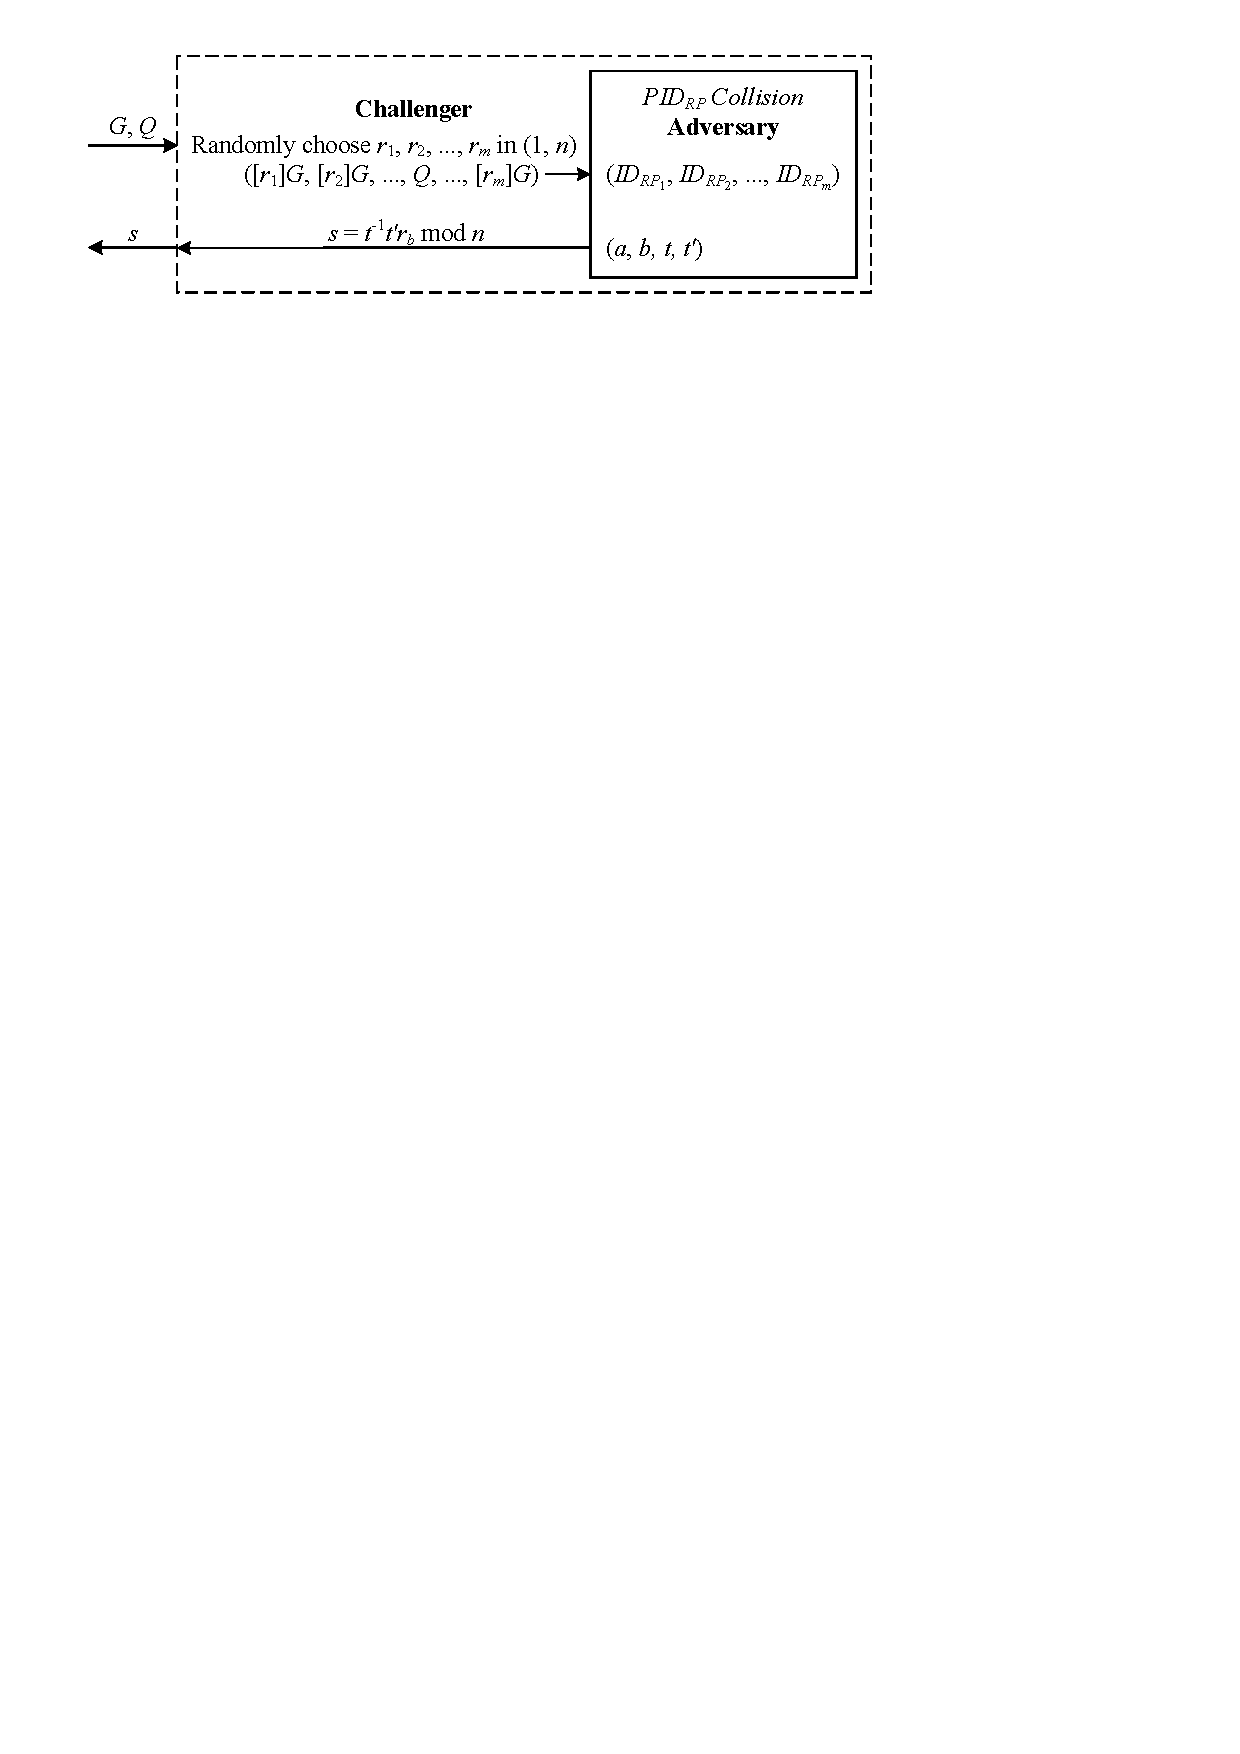
\includegraphics[width=0.97\linewidth]{fig/ecdlp_algorithm.pdf}
  \caption{The PPT algorithm $\mathcal{D}^*_c$ based on the $PID_{RP}$ collision game, to solve the ECDLP}
  \label{fig:ecdlp_algorithm}
\end{figure}

If the adversary succeeds in $\mathcal{G}_c$ and $[r_a]G$ happens to be replaced with $Q$,
 $\mathcal{D}^*_c$ outputs $s=x$ because $[tr_a]G = [t]Q = [t'r_b]G$. For the adversary, $Q$ is indistinguishable from any other RP identities in the input set, as $[r_j]G$ is randomly replaced by the challenger.
Hence, the probability of solving the ECDLP by $\mathcal{D}^*_c$ is formulated as:
\begin{equation*}
{\rm Pr}\{\mathcal{D}^*_c(G, [x]G)=x\} = {\rm Pr}\{s = x\}={\rm Pr}\{a=j\}{\rm Pr}_s=\frac{1}{m}{\rm Pr}_s
\end{equation*}

\newc
If the adversary have advantages in $\mathcal{G}_c$ to find $t$ and $t'$ satisfying $[t]ID_{RP_j} = [t']ID_{RP_{j'}}$,
    ${\rm Pr}_s$ will be non-negligible regardless of $k$.
Therefore, we find that
${\rm Pr}\{\mathcal{D}^*_c(G, [x]G)=x\}$ will become non-negligible as $m$ is a finite integer and $m \ll 2^k$, when $k$ is sufficiently large.
\oldc
This violates the ECDLP assumption. Thus, the probability of finding $t$ and $t'$ that satisfy $[t]ID_{RP_j} = [t']ID_{RP_{j'}}$ in \usso~is negligible. \hfill $\square$


\newc
\vspace{1mm}
\noindent\textsc{Theorem 2. (User Identification)} {\em $PID_U$ in $TK$ uniquely identifies an account at the RP designated by $PID_{RP}$, and this account is uniquely mapped to a user with $ID_U$.}

%In the identity token binding $PID_U$ and $PID_{RP}$, the user pseudo-identity $PID_U$ identifies the authenticated user with $ID_U$, % as $Acct = [ID_U][ID_{RP}]$,
%and only this user,  at the target RP with $ID_{RP} = [r]G$.}
%That is, in UPPRESSO, $Acct$ identifies the mapping $[ID_u][ID_{RP}]$.

\vspace{0.75mm}
\noindent\textsc{Proof.}
To issue an identity token requested for $PID_{RP}$,
    the honest IdP calculates $PID_U = [ID_U]PID_{RP}$ following Equation \ref{equ:PIDU} after authenticating the user with $ID_U$,
and the designated RP calculates $Acct = [t^{-1}]PID_{U} = [ID_U]ID_{RP}$ following Equation \ref{equ:AccountNotChanged}.
$Acct = [ID_U]ID_{RP}$ is a \emph{permanent} identifier determined when the RP and the user register at the IdP,
so $PID_U$ in $TK$ always identifies $Acct$ at the RP and $Acct$ is mapped to a user with $ID_U$.

Next, we prove that it \emph{uniquely} identifies one user in the system and one account at the RP.
Since $\mathbb{E}$ is a finite cyclic group, $ID_{RP} = [r]G$ is also a generator on $\mathbb{E}$ of order $n$. Given a user with $ID_U$, $Acct = [ID_U]ID_{RP}$ is a unique point on $\mathbb{E}$ for $1 \leq u < n$, which is uniquely associated with $ID_U=u$. \hfill $\square$

%According to the \dy~model, the RP may receive a $TK$ issued for another RP from a malicious RP script. However, if $PID_{RP} = [t]ID_{RP}$ holds, the RP can verify its designation by $PID_{RP}$ based on Theorem 1 and associates both $t$ and $TK$ with the current login instance.
%Then, the RP can calculate $Acct$ using $t$ and $PID_U$ following Eq.~\ref{equ:Account}. $Acct$ is determined only by $ID_U$ and $ID_{RP}$ based on Eq.~\ref{equ:AccountNotChanged}, which are permanent identifiers issued by the IdP during registration. Hence, $Acct$ cannot be manipulated by adversaries and is independent of login instances. Therefore, in a user's multiple login instances to the same RP, $PID_U$s are always mapped to one and only one $Acct$ at that RP.

%The detailed process of proof is shown in Appendix.

\newc
\vspace{1mm}
\noindent\textsc{Theorem 3. (Identity Token Integrity)} {\em An identity token $TK$ issued by the IdP cannot be forged or manipulated by any adversaries.}

%{\em Consider an arbitrary identity token $TK$ binding $PID_{RP}$ and $PID_U$. An honest RP accepts $TK$ if and only if $TK$ is valid, $PID_{RP}$ designates this RP with $ID_{RP}$, and $PID_U$ uniquely identifies a user account $Acct=[ID_U]ID_{RP}$ at this RP, indicating that $TK$ binds $ID_{RP}$ and $Acct$.}

%An honest RP accepts only identity tokens binding its pseudo-identity $PID_{RP}$ and the authenticated user's pseudo-identity $PID_U$, and actually binding $ID_{RP}$ and $Acct=[ID_U]ID_{RP}$, when $SK$ is held by only the IdP.

\vspace{0.75mm}
\noindent{\textsc{Proof.} Identity tokens are generated and signed by the honest IdP using its private key.
 $SK$ is protected well at the IdP against adversaries.
%Meanwhile, the IdP's public key $PK$ is sent from the IdP to the RPs.
%and $PK$ which is pre-installed by an RP cannot be manipulated by adversaries.
With the pre-installed $PK$, an RP verifies the identity tokens it receives.
So any forged or manipulated identity token will be rejected.  \hfill $\square$

%Due to the one-to-one mapping between (\emph{a}) the pair of $Acct$ and $PID_{RP}$ and (\emph{b}) the triple ($PID_U$, $PID_{RP}$, $t$), $TK$ binds $ID_{RP}$ and $Acct$ implicitly. \hfill $\square$

% A signed identity token binds $PID_{RP} = [t]ID_{RP}$ and $PID_U = [ID_U]PID_{RP}$, % $Acct$ and $ID_{RP}$ implicitly,
% and any breaking results in some failed checking or verification in the login flow as below.
%First of all, the identity token is signed by the honest IdP using $SK$ and verified by the RP using $PK$, so any modification will be rejected by the RP.
% According to the proof of RP designation, % there is no $t' \neq t$ but satisfying that $PID_{RP} = [t]ID_{RP_j} = [t']ID_{RP_{j'}}$.
% $PID_{RP}$ identifies only the RP with $ID_{RP}$; according to the proof of user identification, $PID_U$ identifies only the user with $Acct = [ID_U]ID_{RP}$ at the RP.
%Therefore, the identity token explicitly binding $PID_U$ and $PID_{RP}$, matches \emph{only} one $ID_{RP}$ and \emph{only} one $Acct = [t^{-1}]PID_{U}$.
%Therefore, $Acct$ and $ID_{RP}$ are actually bound in the token by the IdP's signatures,


\vspace{1mm}
\noindent{\textsc{Theorem 4. (Identity Token Confidentiality)}} {\em An identity token $TK$ %whose $PID_{RP}$ designates an RP with $ID_{RP}$ can
is accessible to the designated RP, besides the requesting user and the IdP.}
%An identity token is accessible to only the authenticated user and the target RP, in addition to the IdP signing this token.

\vspace{0.75mm}
\noindent\textsc{Proof.}
An identity token is generated by the IdP and then sent to the requesting user (i.e., its IdP script).
 The IdP script forwards the token to the RP script, which should be downloaded from the origin of $Enpt_{RP}$ which is specified in a verified RP certificate.
The IdP script calculates $PID_{RP}$ based on $ID_{RP}$ bound in this RP certificate,
    so this RP is designated in the identity token.

All the communications between the IdP, RPs, and users are protected by HTTPS
 and two scripts communicate with each other through dedicated \verb+postMessage+ HTML5 channels.
According to the conclusions of the DYU model, 
 the identity tokens are not leaked to any adversaries. \hfill $\square$


\vspace{1mm}
\noindent\textsc{Theorem 5. (Security)} {UPPRESSO is secure.}

\vspace{0.75mm}
\noindent\textsc{Proof.}
According to the formal analysis \cite{SPRESSO,FettKS14},
    an SSO system is secure, if (\emph{a}) an adversary never presents an identity token that is accepted by an honest RP to derive an honest user's account at this RP
    and (\emph{b}) an honest user never presents an identity token that is accepted by an honest RP to derive another user's account at this RP.

%In a secure SSO that is robust against impersonation attacks, an honest user should be able to prove her identity to the target RP with an identity token issued by the IdP. As pseudo-identities are used in \usso, an RP needs to verify that ({\em a}) $PID_{RP}$ in the received identity token is a transformation from its own $ID_{RP}$ and tied to the current login instance, which requires {\em RP designation}; and ({\em b}) $PID_U$ included in the identity token can be associated with a unique, long-term user account it maintains, which requires {\em user identification}. Besides, the identity token for an honest RP should not be intercepted by malicious users or RPs, requiring the {\em confidentiality of identity tokens}, nor be forged or tampered with to include a fake $PID_U$ or $PID_{RP}$, requiring the {\em integrity of identity tokens}.

When confidentiality and integrity of identity tokens is satisfied,
    an adversary cannot presents an identity token issued for honest users and accepted by an honest RP.
When RP designation and user identification are satisfied,
    an identity token issued to an adversary always derives the adversary's account at any RP.
So an adversary never presents an identity token that is accepted by an honest RP to derive an honest user's account at this RP.

%Meanwhile, $PID_U$ can only be calculated by the IdP and the user, since no one else knows or could intercept $u$ according to the DYU model. \oldc

According to the conclusions of the DYU model,
    $PID_U$ is calculated based on the user when the IdP issues an identity token for an authenticated user.
Moreover, because confidentiality and integrity of identity tokens are satisfied,
    an honest user never presents a token issued for other users and accepted by an honest RP.
When user identification user is satisfied,\footnote{It is worthy noting that RP designation is a precondition of user identification in UPPRESSO. In other SSO systems, RP designation is not always a precondition of user identification.}
    this token always derives this honest user's account.
\hfill $\square$

%Finally, according to Theorems 1, 2, 3, 4 and 5, UPPRESSO is secure.

\subsection{Privacy}
\label{sec-:analysis}
In this section, we show that \usso~can effectively prevent privacy threats introduced by IdP-based login tracing and RP-based identity linkage.

\newc In each login instance, the IdP receives an identity-token request from the user (Step 3.1 in Section~\ref{implementations}), which reveals only the user's identity and the RP's pseudo-identity $PID_{RP}$. To prove that the IdP cannot trace one user's multiple logins to different RPs, we need to show that these $PID_{RP}$s are \emph{indistinguishable}.

\vspace{1mm}
\noindent{\textsc{Theorem 5. (Privacy against the IdP)}} {\em Consider $PID_{RP} = [t]ID_{RP}$, where $t$ is random in $\mathbb{Z}_n$ and unknown to the IdP. The IdP is unable to distinguish the pseudo-identities of RPs in identity-token requests made by honest users.}

\vspace{0.75mm}
\noindent{\textsc{Proof.} Consider a user's two arbitrary logins to an RP where $PID^{i}_{RP} = [t]ID_{RP}$ and $PID^{i'}_{RP} = [t']ID_{RP}$, and the same user's login to another RP where $PID^{i''}_{RP'} = [t'']ID_{RP'}$. As stated in Theorem 2, $ID_{RP} = [r]G = Q$ and $ID_{RP'} = [r']G = P$, where $P$ and $Q$ are two different points on the curve $\mathbb{E}$. According to the \dy~model, $t$, $t'$, and $t''$ are randomly selected by the IdP script and shared only with the corresponding RP through the RP script, they are unknown to the IdP. Therefore, in the IdP'view, $[t]Q$, $[t']Q$, and $[t'']P$ are three random points on $\mathbb{E}$ and they are indistinguishable from each other. \hfill $\square$

%as well as from a $PID_{RP}$ generated in an arbitrary login instance for an arbitrary user to log in to an

%\textcolor{blue}{The information accessible to the IdP and derived from the RP's identity, is only $PID_{RP}$ in identity-token requests, where $PID_{RP} = [t]ID_{RP}$ is calculated by a user. % and $t$ is kept secret to the IdP.
%So the prevention against the IdP-based login tracing in UPPRESSO is expressed formally as below.}

% \vspace{1mm}
% \noindent\textcolor{blue}{\textbf{Privacy against the IdP.}~~If $t$ is random in $\mathbb{Z}_n$ and unknown to the IdP, the IdP cannot infer any information about $ID_{RP_j}$ or link any pair of $PID_{RP_j}^i$ and $PID_{RP_{j'}}^{i'}$ ($i \neq i'$ but $j = j'$), from a user's identity-token requests for $PID_{RP_j}^i$ ($i,j = 1, 2, \cdots$).}

% \vspace{0.75mm}
% \noindent\textbf{Proof.}
% Because (\emph{a}) $ID_{RP} = [r]G$ is also a generator of order $n$, where $G$ is a generator of finite cyclic group $\mathbb{E}$ \textcolor{blue}{and (\emph{b}) $t$ is a random number in $\mathbb{Z}_n$ and kept unknown to the IdP,} from the IdP's view,
%  $PID_{RP}$ is \emph{indistinguishable} from a random variable on $\mathbb{E}$.
% Thus, the IdP cannot infer any information about $ID_{RP}$ from $PID_{RP} = [t]ID_{RP}$, or distinguish $[t]ID_{RP_j} = [tr]G$ from any other $[t']ID_{RP_{j'}} = [t'r']G$. So the IdP-based login tracing is impossible. $\square$

Next, we show that \usso~protects user privacy against RP-based linkage. This is to prove that the colluding RPs have limited knowledge about the users who have authenticated with them (using $PID_U$s). Even if they share this information, it is insufficient to distinguish the pseudo-identities of the users nor link the ones belonging to the same user. In Section~\ref{implementations}, we show that the RP receives $t$ (Step 2.1) and the identity token (Step 4.1) from which it can extract $PID_{RP}$ and $PID_U$. Meanwhile, the RP knows its own $ID_{RP}$ and the accounts of its users (i.e., $Acct$s), %Since $PID_{RP}= [t]{ID_{RP}}$ and $Acct = [t^{-1}]PID_{U}$, we can deduce $PID_{RP}$ and $PID_U$ from $ID_{RP}$ and $Acct$ with a valid $t$.
where $PID_{RP}$ and $PID_U$ can be deduced from $ID_{RP}$ and $Acct$ with a valid $t$, respectively. Therefore, when user $U_i$ requests to log in to $RP_j$, the RP's knowledge can be defined as $L_{i, j}=(ID_{RP_j}, t_{ij}, Acct_i)$. %According to Equation~\ref{equ:Account}, we have $L_{i, j}=([r_j]G, t_{ij}, [u_ir_j]G)$.

Now, let us consider $v$ malicious users who have logged in to $c$ colluding RPs. Each RP has collected information about $v$ login instances and shared it with each other. We denote this shared knowledge as:
\begin{equation*}
\mathfrak{L}=\left\{ \begin{matrix}
L_{1,1}, & L_{1,2}, & \cdots, & L_{1,c}\\
L_{2,1}, & L_{2,2}, & \cdots, & L_{2,c}\\
\cdots, & \cdots, & \cdots, & \cdots\\
L_{v,1}, & L_{v,2}, & \cdots, & L_{v,c}
\end{matrix}\right\}
\end{equation*}
where $L_{i, j}=(ID_{RP_j}, t_{ij}, Acct_i)=([r_j]G, t_{ij}, [u_ir_j]G)$ according to Equation~\ref{equ:Account}.

\vspace{1mm}
\noindent{\textsc{Theorem 5. (Privacy against Colluding RPs)}} {\em Consider $PID_{RP} = [t]ID_{RP}$, where $t$ is random in $\mathbb{Z}_n$ and unknown to the IdP. The pseudo-identities of RPs in the identity-token requests from honest users are indistinguishable to the IdP.}


\oldc

% \vspace{1mm}
% In every login instance, without knowing $u$ and $r$, an RP holds $ID_{RP}$ and $Acct$, receives $t$, calculates $PID_{RP}$, and verifies $PID_{RP}$ and $PID_U$ in the identity token. After filtering out the redundant information (i.e., $PID_{RP}= [t]{ID_{RP}}$ and $Acct = [t^{-1}]PID_{U}$), the RP actually receives $(ID_{RP}, t, Acct) = ([r]G, t, [ur]G)$. Therefore, in \usso~the prevention against the RP-based identity linkage is expressed as follows.

% \vspace{1mm}
% \noindent\textcolor{blue}{\textbf{Privacy against Colluding RPs.}~~Provided that $u$ and $r$ are kept unknown to RPs,
% based on the collected information of login instances by $v$ users,
% $c$ colluding RPs cannot decide whether a login instance to another RP is initiated by one of these $v$ users or not,
%     where
%     the collected login instances are denoted as $\mathfrak{L}=\left\{ \begin{matrix}
% L_{1,1}, & L_{1,2}, & \cdots, & L_{1,c}\\
% L_{2,1}, & L_{2,2}, & \cdots, & L_{2,c}\\
% \cdots, & \cdots, & \cdots, & \cdots\\
% L_{v,1}, & L_{v,2}, & \cdots, & L_{v,c}
% \end{matrix}\right\}$, $L_{i, j} = (ID_{RP_j}, t_{i, j}, [ID_{U_i}]{ID_{RP_j}}) = ([r_j]G, t_{i,j}, [u_ir_j]G)$,
%     and the login instance to $RP_{c+1}$ is $L'=(ID_{RP_{c+1}}, t', [ID_{U'}]ID_{RP_{c+1}}) = ([r_{c+1}]G, t', [u'r_{c+1}]G)$.}


\vspace{0.75mm}
\noindent\textbf{Proof.}
We prove this privacy property,
 based on the elliptic curve decisional Diffie-Hellman (ECDDH) assumption. %\cite{GoldwasserK16}.
%That is, while there is the login to an RP, for colluded RPs, they cannot decide whether this login and any logins to other RPs are from the same user.
%
Let $\mathbb{E}$ be an elliptic curve,
    and $G$ be a point on $\mathbb{E}$ of order $n$.
For any PPT algorithm $\mathcal{D}$, the probability of distinguishing
 $([x]G$, $[y]G$, $[xy]G)$ and $([x]G$, $[y]G$, $[z]G)$
is negligible,
 where $x$, $y$ and $z$ are integers randomly and independently chosen in $\mathbb{Z}_n$.
Let  ${\rm Pr}\{\}$ denote the probability and
 we define
\begin{align*}
&{\rm Pr}_1 =  {\rm Pr}\{\mathcal{D}(G, [x]G, [y]G, [xy]G)=1\} \\
&{\rm Pr}_2 =  {\rm Pr}\{\mathcal{D}(G, [x]G, [y]G, [z]G)=1\}
\end{align*}
So $\epsilon_{r}(k) = |{\rm Pr}_1 - {\rm Pr}_2|$ becomes negligible as $k$ increases.

\begin{figure}[tb]
  \centering
  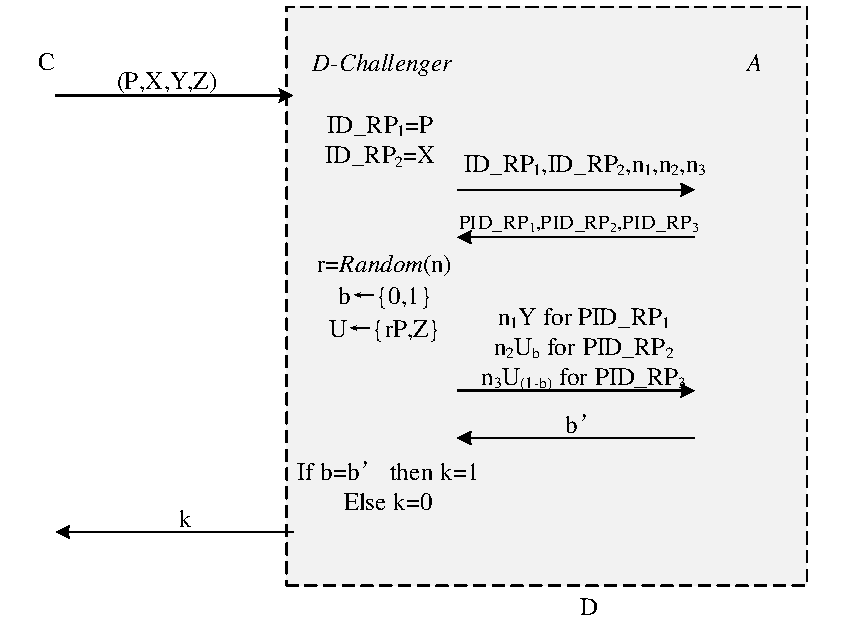
\includegraphics[width=0.97\linewidth]{fig/dalgorithm.pdf}
  \caption{The PPT algorithm $\mathcal{D}^*_r$ based on the RP-based identity linkage game, to solve the ECDDH problem}
  \label{fig:dalgorithm}
\end{figure}

We define the RP-based identity linkage game $\mathcal{G}_r$:
after receiving $\mathfrak{L}$ and $L'$ from a challenger,
    the adversary outputs the result $s = 1$ if it decides $u' \in \{u_1, u_2, \cdots, u_v\}$ or $s = 0$ if $u'$ is randomly chosen in $\mathbb{Z}_n$.
The adversary's advantage in $\mathcal{G}_r$ is defined as $\mathbf{Adv}_{A}$.
%If the adversary is able to distinguish whether $u' \in \{u_1, u_2, \cdots, u_v\}$ or not,
%    the adversary will have non-negligible advantages in $\mathcal{G}_r$
%        and ${\rm Adv}_A$ is non-negligible.
Then,
\begin{align*}
&{\rm Pr}'_1={\rm Pr}\{\mathcal{G}_r(\mathfrak{L}, L'|ID_{U'} \in \{ID_{U_1}, ID_{U_2}, \cdots, ID_{U_v}\})=1\} \\
&{\rm Pr}'_2={\rm Pr}\{\mathcal{G}_r(\mathfrak{L}, L'|ID_{U'} \in \mathbb{Z}_n)=1\}\\
&{\mathbf{Adv}}_{A}=|{\rm Pr}'_1-{\rm Pr}'_2|
\end{align*}

We design a PPT algorithm $\mathcal{D}^*_r$ based on $\mathcal{G}_r$, shown in Figure \ref{fig:dalgorithm}, to solve the ECDDH problem.
The input is in the form of $(G$, $Q_1=[x]G$, $Q_2=[y]G$, $Q_3=[z]G)$.
On receiving the input, the challenger of $\mathcal{G}_r$ randomly chooses
 $\{u_1, u_2, \cdots, u_v\}$, $\{r_1, r_2, \cdots, r_c\}$, $\{t_{1, 1}, t_{1, 2}, \cdots, t_{v, c}\}$, and $t'$ in $\mathbb{Z}_n$.
Then the challenger constructs $\mathfrak{L}$ and $L'$ as below.
It firstly assigns $L_{i, j} = ([r_j]G, t_{i, j}, [u_ir_j]G)$, %$1\leq i \leq v$ and $1\leq j \leq c$,
    and randomly chooses $d \in [1, v]$ to
 replace $[u_d r_j]G$ with $[r_j]Q_1=[xr_j]G$ for $1\leq j \leq c$.
So $\mathfrak{L}=\left \{ \begin{matrix}
L_{1,1},&L_{1,2},&\cdots,&L_{1,c}\\
L_{2,1},& L_{2,2},&\cdots,&L_{2,c}\\
\cdots,&\cdots,&\cdots,&\cdots\\
([r_{1}]G, t_{d, 1}, [r_{1}]Q_1),&\cdots,&\cdots,&([r_{c}]G, t_{d, c}, [r_{c}]Q_1)\\
\cdots,&\cdots,&\cdots,&\cdots\\
L_{v,1},&L_{v,2},&\cdots,&L_{v,c}
\end{matrix}\right\}$.
%$L=$\{($[r_1]G$, $t_{1, 1}$, $[[u_1][r_1]G$), ($[r_2]G$, $t_{1, 2}$, $[u_1][r_2]G$), $\cdots$, ($[r_{\beta}]G$, $t_{\alpha, \beta}$, $[r_{\beta}]Q_1$), $\cdots$, ($[r_b]G$, $t_{a, b}$, $[u_a][r_b]G$)\}
%
The challenger assigns $L' = (Q_2, t', Q_3) = ([y]G, t', [z/y][y]G)$.
Finally,
    $\mathfrak{L}$ and $L'$ are sent to the adversary,
        and the output $s$ of $\mathcal{G}_r$ is output by the challenger.
According to the above construction of $\mathfrak{L}$ and $L'$,
    $x$ is actually inserted into $\mathfrak{L}$ as $u_d$
    and $z/y$ is assigned to $u'$.
So, if $z = xy$, then $z/y=x$ and $ID_{U'} \in \{ID_{U_1}, ID_{U_2}, \cdots, ID_{U_v}\}$;
    otherwise, $ID_{U'} \in \mathbb{Z}_n$.
Thus,
\begin{align*}
&{\rm Pr}_1={\rm Pr}\{\mathcal{D}^*_r(G, [x]G, [y]G, [xy]G)=1\}={\rm Pr}'_1 \\=&  {\rm Pr}\{\mathcal{G}_r(\mathfrak{L}, L'|ID_{U'} \in \{ID_{U_1}, ID_{U_2}, \cdots, ID_{U_v}\})=1\} \\
&{\rm Pr}_2={\rm Pr}\{\mathcal{D}^*_r(G, [x]G, [y]G, [z]G)=1\} ={\rm Pr}'_2 \\=&  {\rm Pr}\{\mathcal{G}_r(\mathfrak{L}, L'|ID_{U'} \in \mathbb{Z}_n)=1\}\\
&{\mathbf{Adv}}_{A}=|{\rm Pr}'_1-{\rm Pr}'_2|=|{\rm Pr}_1-{\rm Pr}_2|=\epsilon_{r}(k)
\end{align*}

The ECDDH assumption means that in $\mathcal{G}_r$ the adversary does not have advantages,
    i.e., cannot distinguish a user $U'$ chosen from \{${U_1}, {U_2}, \cdots, {U_v}$\}
        or randomly from the universal user set.
%    (indistinguishability of users to colluding RPs).
So the RP-based identity linkage is impossible. $\square$
